
Next step was to do the analysis on the bigger scale and see if sentiment changes with the amount of releases/commits per month. For this, I'm going to use tweets collected with period one week. The classifier used is completely the same so there should not be big differences in the sentiment of the same projects. Results can be seen in table \ref{table:weeklyAverageTable} and figure \ref{fig:weeklyAverageBarchart}

\begin{table}[H]
\centering
\begin{tabular}{ |p{3cm}|p{3cm}|p{3cm}|}
 \hline
\textbf{Project }& \textbf{Average sentiment}\\
 \hline
 NodeJS   & 0.697 \\ \hline
 EmberJS   & 0.709\\ \hline
 VueJS   & 0.715 \\ \hline 
 Symfony & 0.727 \\ \hline   
 AngularJS   & 0.727 \\ \hline
 CakePhp & 0.703 \\ \hline 
 Bower   & 0.641 \\ \hline 
 Laravel & 0.701 \\ \hline
 Gulp & 0.578 \\ \hline
 Yii & 0.658 \\ \hline
 Bootstrap & 0.713 \\ \hline
\end{tabular}
\caption{Average sentiment of tweets 3 days before and after releases}
\label{table:weeklyAverageTable}
\end{table}


\begin{figure}[H]%
    \centering
	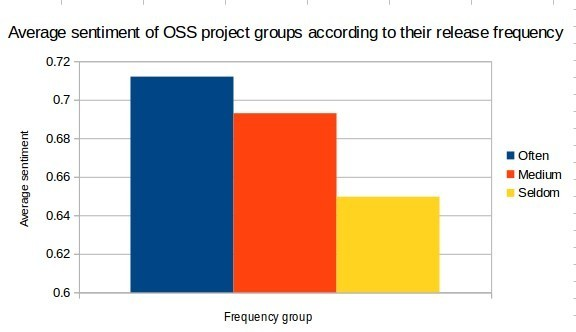
\includegraphics[width=12cm]{weeklyAverageBarchart.jpg}
    \caption{Average sentiment of OSS project groups according to their release frequency}%
    \label{fig:weeklyAverageBarchart}%
\end{figure}

In both of previous analysis, I've used the simplest aggregation operation which is average. Replacing this one with median, modus or some more advanced aggregations could potentially yield different results but because each group is represented just by 3 or 4 OSS projects, losing any data would actually be a significant part of the overall analysed dataset. Using more projects could be potentially a part of future work.